\chapter{Prestudy}
\label{chap:prestudy}
\section{Children with asthma}
Asthma is a chronic lung disease that alot of people suffer from. It is often more prominent in children, who are more active and easily exited then
adults. The asthma is typically triggered by exitement, physical activity, rashes or allergies. The problem is managed by multiple medicines, 
with different schedules as to when to take them depending on the condition of the child. There are inhalation medicines that consists of either 
small dustparticles that effect the lungs locally, or saltwater that are inhaled as vapor, either alone or combined with other medicines to loosen 
up slime. There are also pills or liquid medicines that either affects the immune system or affects the body globally, not just locally in the lungs.

The medicines can also be divided into medicines that have immidiate effects, and are used during an asthma attack, while other medicines are preventive, 
and is taken on a regular schedule. In addition you have preventitive medicines targeted at bolstering your immune system before going to areas or days
where the child is likely to be in contact with materials it is alergic to.	

With some of the inhalationmedicines it's difficult to time the inhalation with the release of medicine, and here an inhalation chamber, or inhalation 
mask, is used. When the child has taken the nebulizer this way, that is usually taken once or twice a day, they must remember to wash their mouth. 

\section{Parents with children affected by asthma}

Parents of children with asthma face a series of challenges concerning the medicination of their children. 
One of these challenges is to give the correct amount of medicine, the right type of medicine, at the 
correct time of the day. Many parents have experienced stressful mornings where they are late for work, 
their children is unwilling to take their medicine and they either do it in an incorrect way, reducing the 
medicines effect, or not at all. The medication plans can be hard to understand, even though they are 
designed to be easy, and it's typically only one of the parents that have gotten the instructions from 
the doctor directly, and it becomes even harder for the other one to do it correctly.

The children isn't always happy about taking their medicine. The inhalation mask might be scary, the 
medication might interfere with their planned activities that day, or any number of other reasons the child 
might not want to take his medicine that day. Having to force a child to take their medicine could make the 
child associate taking the medicine with a negative experience, and it becomes increasingly difficult to 
give the medicine to the child. 

\section{The concept of gamification}

Gamification is the concept of applying game-design thinking to non-game applications to make them more fun and engaging. The term
was first mentioned in March 2004, but was not popular before 2010. By using gamification, we hope to make asthma treatments for children
more enjoyable to do.


There exists a lot of common techniques applied to introduce gamification to a process. These techniques include, but are not limited to:
\begin{itemize}
  \item Achievements/badges
  \item Levels
  \item Leaderboards
  \item Progress bars
  \item Avatars
  \item Gifting
  \item Challenges
  \item Embedding of minigames
\end{itemize}

These techniques are all widely used. Here are some examples:
\begin{itemize}
  \item Games for PlayStation and XBOX are more used online now, and fewer people are playing thos game offline.
   To make people finish the campaign the these games, they are using trophys to motivate people to complete games 100\%. 
   You may have to collect every single item in the game, fight every boss and so on.
  \item Nike+ introduced gamification to training. You can track how fast you run, your maximum pulse and so on, and try to beat this target the next time you are running.
  \item You ``check in'' to places you have been with Google Maps.  
  \item Airline companies uses points as bait for customers to fly more with a company. At a certain level of these points, you may get one more flight for free, get a free upgrade to a better seat
  and so on. 
\end{itemize} 

%Kanskje skrive om dette?
As previously mentioned, we hope gamification will help making children's treatment as enjoyable as possible. Michael Wu (Ph.D in Biophysics) has proven that gamification has an impact on human motivation. 
As Michael Wu presents it:
``Game mechanics and game dynamics are able to positively influence human behavior because they are designed to drive the players above the
activation threshold (i.e. the upper right of the ability-motivation axis), 
and then trigger them into specific actions'' (Wu, 2011).  
Game mechanics have been proven to positively influence human behaviour, because these game mechanics are designed to drive the players ab
%Referanser: gamification.org, Gamification 101 (se bibliografi)


Even though gamification has a lot of positive sides, it has a bad side if gamification is done the wrong way.
The fact that we are using gamification to motivate children, it makes it even worse. If children feels that
they are stuck in a game, motivation may very easily be broken down. So whatever concept we come up with, it has to be 
to motivate the children at all time. They cannot feel stuck with our concept. This concept is up to the customer to create, 
while we will be implementing it.  

\section{Karotz}
Karotz.com (2012)\cite{karotz} describes Karotz as a robot shaped 
as a bunny that can interact with
a user through light, ear movement and sound. It can also take
input through a button, moving its ears, an RFID (Radio-frequency identification) chip, voice
commands and serial (Internet) communication.

The project includes developing an application for the Karotz
platform that will serve as an addition to the mobile applications.
It is therefore necessary to study its interfaces, development
methods and API of the machine.

\begin{figure}[h]
	\centering
		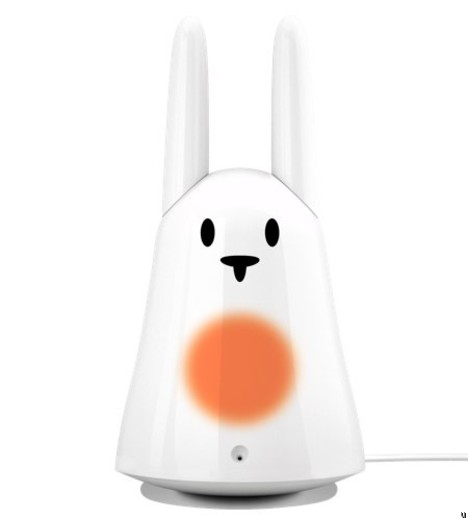
\includegraphics[height=10cm]{Pictures/karotzimg}
	\caption{Karotz: A bunny-shaped robot}
	\label{fig:karotz}
\end{figure}

\subsection{Application Platform}
Karotz application (called ``Appz'') are installed through an
online platform located on the Karotz web site. They can be
launched on the Karotz itself either through a scheduler, voice
commands or an RFID chip. These RFID chips come in various shapes,
sizes and colors. Figure \ref{fig:flatnanoz} and Figure 
\ref{fig:nanoztag} show examples of the different kinds of ``nanoz'',
that are small figures with an integrated RFID chip.

\begin{figure}
	\begin{minipage}[b]{0.4\linewidth}
		\centering
			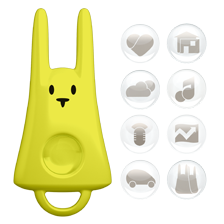
\includegraphics[width=0.30\paperwidth]{Pictures/FlatnanozYellow}
		\caption[Flatnanoz]{A flat nanoz--flatnanoz-- a figure with an RFID chip used to provide input to a Karotz.}
		\label{fig:flatnanoz}
	\end{minipage}
	\hspace{3cm}
	\begin{minipage}[b]{0.4\linewidth}
		\centering
			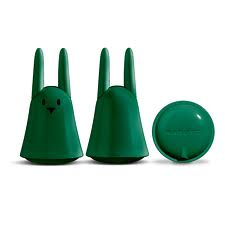
\includegraphics[width=0.30\paperwidth]{Pictures/NanoztagGreen}
		\caption[Nanoztag]{A round nanoz--nanoztag-- a figure with an RFID chip used to provide input to a Karotz.}
		\label{fig:nanoztag}
	\end{minipage}
\end{figure}

Some mentionable applications made by other developers are 
``At Home'', an application that may register that someone checks 
in at the Karotz, and send an e-mail to a predetermined mail 
address, so children may tell their parents that they are home. 
``Twitter for Karotz'' may read you tweets and post tweets based 
on voice-commands. Another mention is ``Weather'' which may tell 
you the forecast for the day or the following day. It seems all 
applications registered at the Karotz website are fairly simple 
and have little functionality.

As for launching the BLOPP application, the times for the scheduler must
be manually set through the Karotz web site, so it cannot be 
used for notifications directly. The best option for the BLOPP 
implementation would therefore be to set a scheduler to start
every day at 00:00 and stop every day at 23:59. This way it can
be ensured that the application is always running, updating
itself with medications, status and times, and a timer can be
used to schedule notifications.

%\subsection{The two APIs}
The Karotz can be programmed in two different ways: either
through a web REST (Representational State Transfe) framework, 
or with JavaScript that runs as an embedded program on the robot itself.

The requirement that a REST program would have to be hosted
somewhere, combined with the fact that an embedded program 
provides more flexibility in terms of local storage to limit the
amount of information sent over a network makes the JavaScript
framework a more suitable choice for the BLOPP project.

%\subsection{Karotz Output Channels}
The Karotz has a few ways of providing output to the end-user. It
can be asked to
\begin{itemize}
    \item play sound files;
    \item move its ears;
    \item speak, using a TTS (text-to-speach) engine;
    \item illuminate its stomach in different colors;
    and
    \item communicate over the internet with HTTP (Hyper Text Transfer Protocol) GET and POST 
          methods.
\end{itemize}

For providing user commands, TTS could be an option if the engine
supported Norwegian, but since the language options are limited to
English, French, German and Spanish, speech will have to be
created by recording sound files and playing them with the
multimedia engine.



 
